\clearpage
\section{Ablation of Prelude Normalization}
\label{sec:prelude-norm}

In our initial set of experiments, we found that Parcae was able to train stably on the 140M, 370M, and 770M model configurations. Unfortunately, at the 1.3B scale, training appeared stable for the first 150k optimizer steps, afterwards exhibited state explosion and loss spikes, an observation which can be made in \cref{fig:prelude-instability}. To diagnose and fix these issues, we performed a deep exploration of the weight checkpoints before and during loss spikes, investigating both dynamical systems parameters (e.g., $\A, \B, \C, \dt$) and non-linear parameters $\overline{\mathcal{R}}$.

\begin{figure}[!h]
    \centering
    \vspace{-0.5em}
    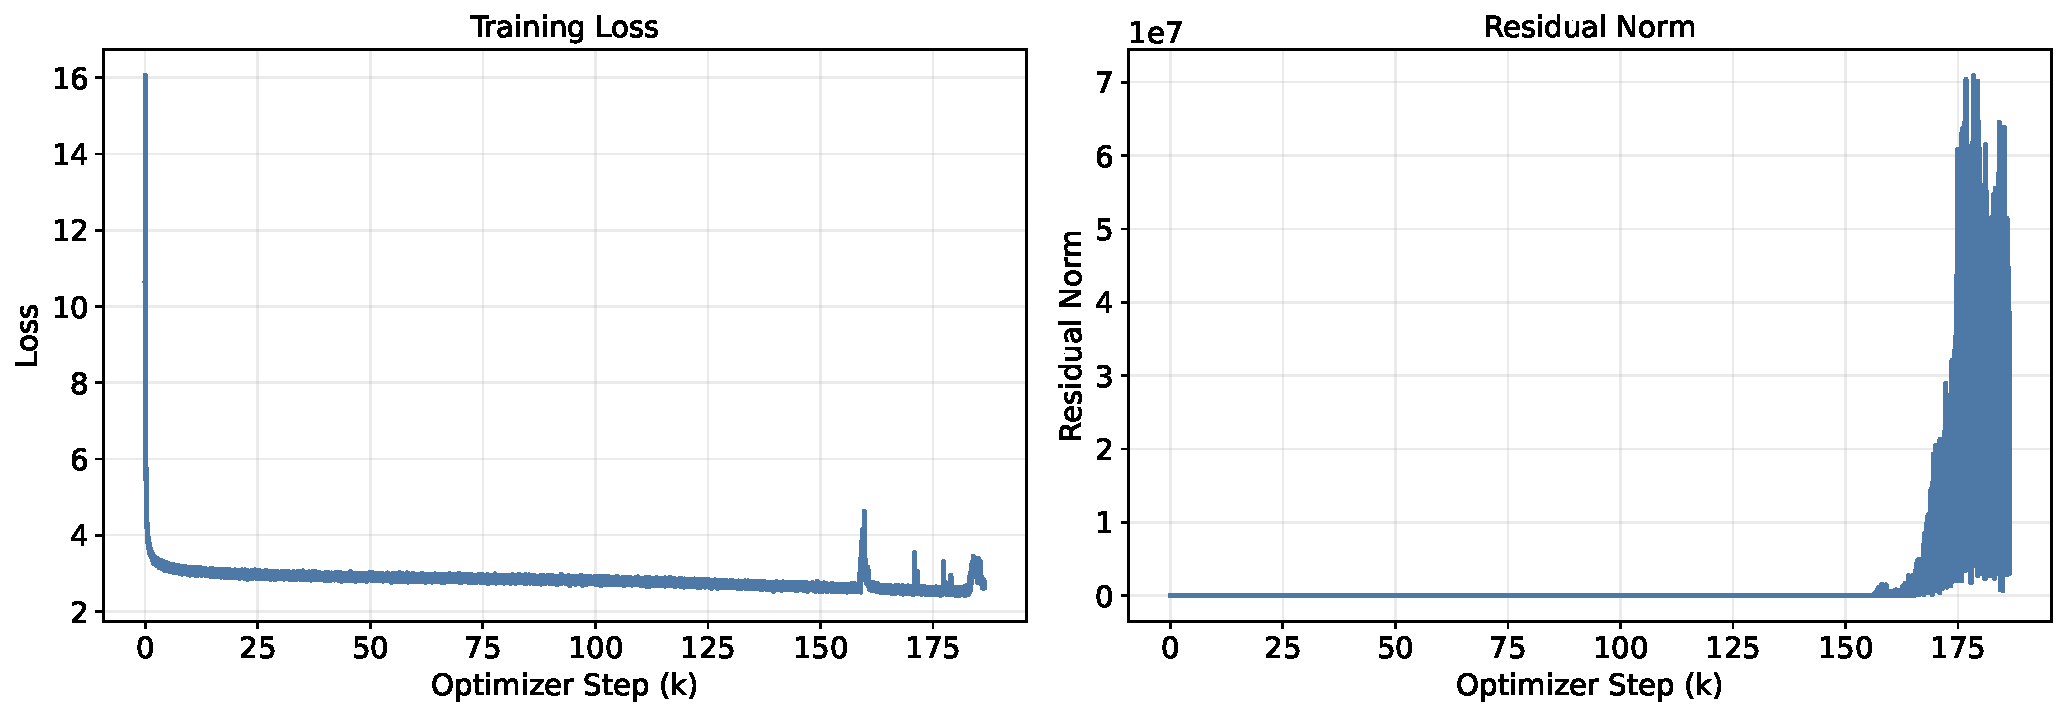
\includegraphics[width=\linewidth]{figures/appendix/prelude_norm.pdf}
    \vspace{-2em}
    \caption{\textbf{Late Stage Instability of 1.3B Parcae models.} We observe loss spikes and state explosion at the final stages of our large-scale run.}
    \label{fig:prelude-instability}
\end{figure}


\begin{figure}[!h]
    \centering
    \vspace{-0.5em}
    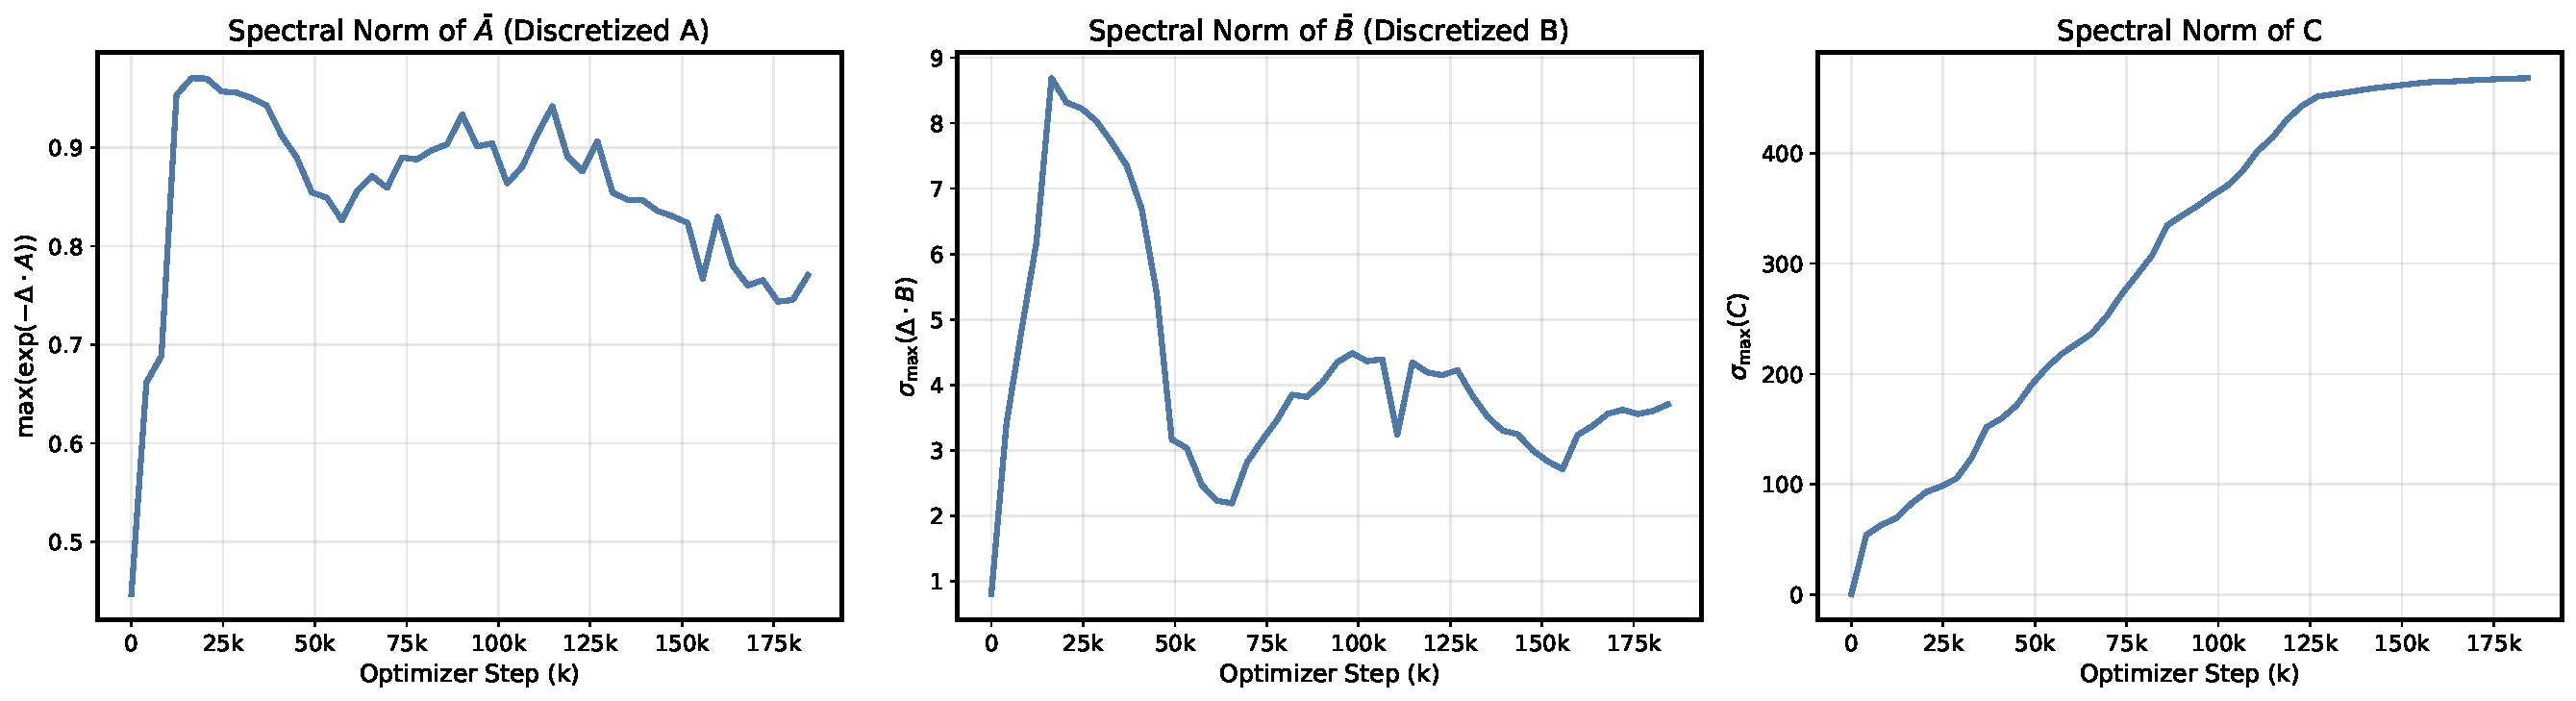
\includegraphics[width=\linewidth]{figures/appendix/spectral_norms_ABC.pdf}
    \vspace{-2em}
    \caption{\textbf{Spectral Norms of $\dA, \dB, \C$ throughout training 1.3B Parcae.} We find that the spectral norm of $\dA$ and $\dB$ remain stable throughout training, while the spectral norm of $\C$ grows.}
    \label{fig:abc_spectral}
\end{figure}

We begin by exploring the spectral norm of $\dA$, $\dB$, $\C$ to see if our dynamical systems block was creating instability, results of which can be found in \cref{fig:abc_spectral}. While we observe that the spectral norm remains relatively low for $\dA$ and $\dB$, we observed that the spectral norm of $\C$ grew significantly throughout training. While this could be concerning, we find that when passing real activations to $\C$, using a subset of the validation set, the empirical expanse ratio $\frac{||C(x)||}{||x||}$ (i.e., how much the norm of the residual $x$ grew after performing $\C(x)$) remained relatively low, as seen in \cref{fig:c_expansion}.


\begin{figure}[!h]
    \centering
    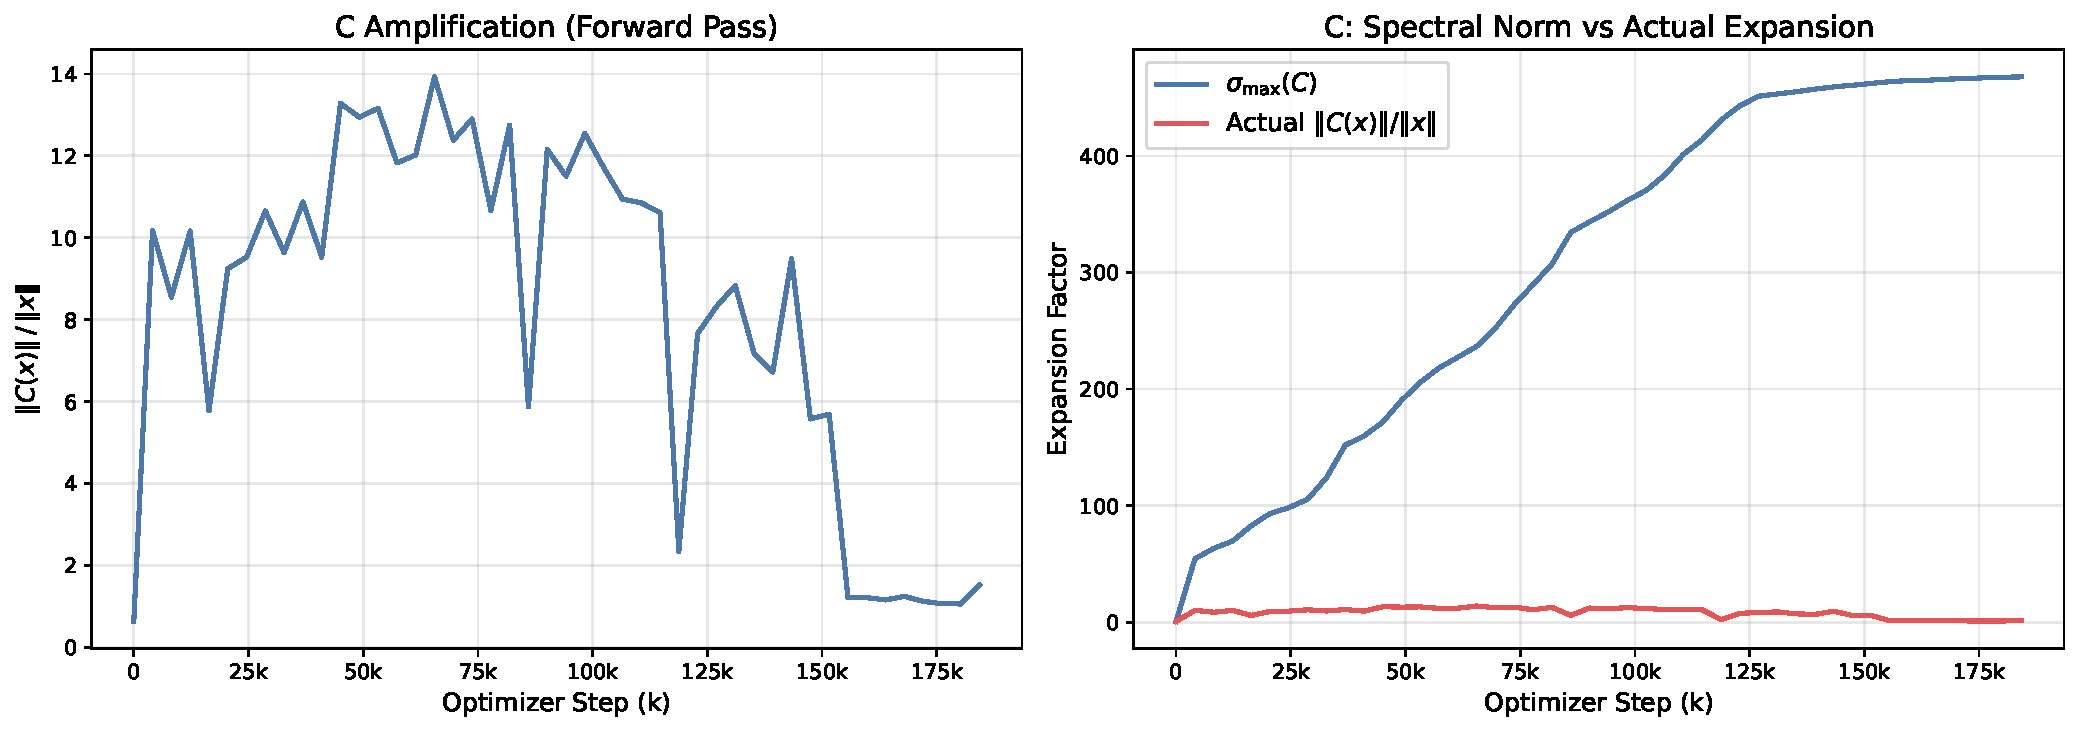
\includegraphics[width=\linewidth]{figures/appendix/C_expansion.pdf}
    \caption{\textbf{Comparison of $\C$ Amplification with Spectral Norm.} We observe that the actual expansion ratio of $\C$ is small and decreasing slowly throughout training.}
    \label{fig:c_expansion}
\end{figure}


\begin{figure}[!h]
    \centering
    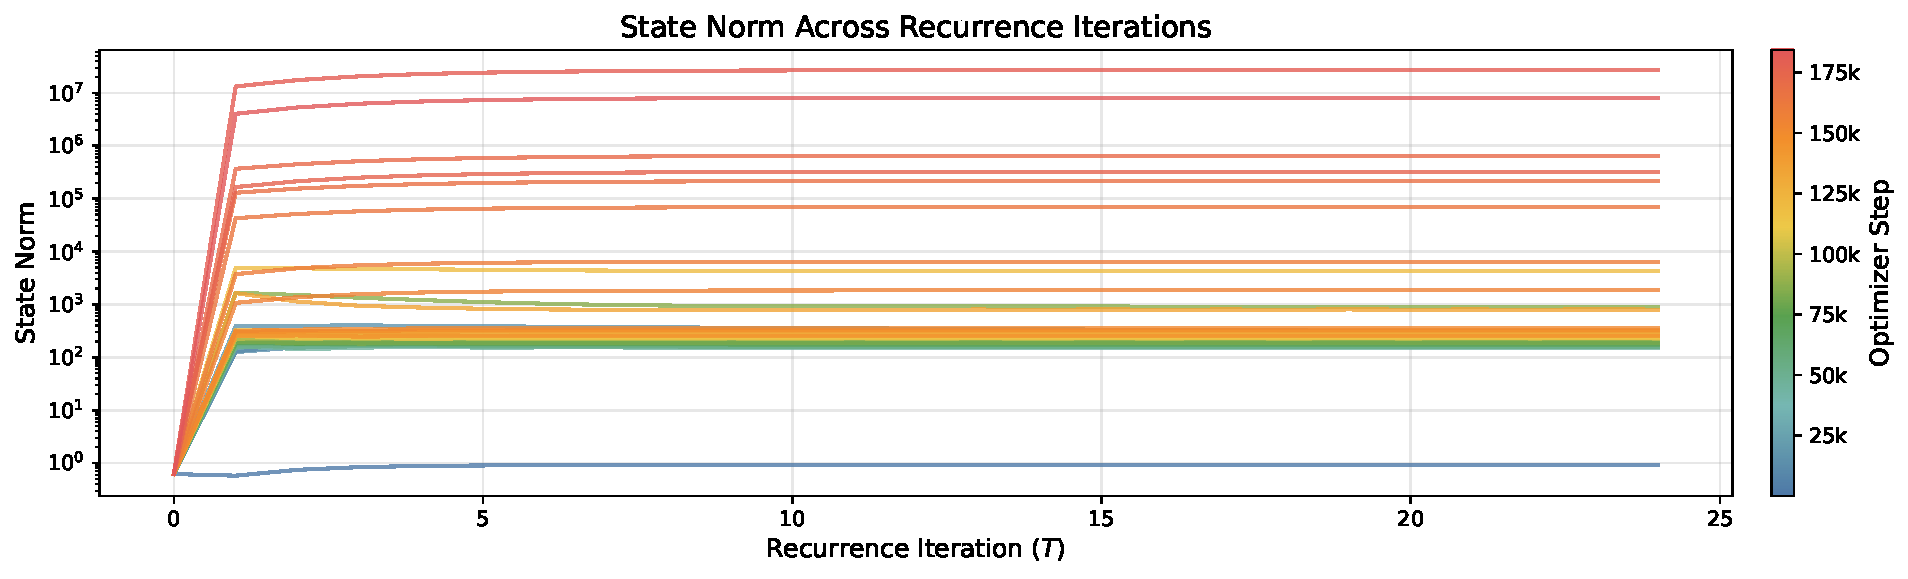
\includegraphics[width=\linewidth]{figures/appendix/state_norm_per_iteration.pdf}
    \caption{\textbf{Empirical Average of Recurrent State Norm over $T$ iterations.} For each checkpoint we have for our failed 1.3B Parcae model run, we evaluate the recurrent norm through $T=24$ recurrences at test time, on a held out validation set of fineweb-edu \cite{penedo2024finewebdatasetsdecantingweb}. We find that after an initial explosion on the first recurrence, the state remains relatively stable.}
    \label{fig:state_norm_diagnose}
\end{figure}

These results indicate that the dynamical systems units are likely not causing an explosion, and thus, we turn our exploration of the dynamics of the entire recurrent unit. Specifically, we track the recurrent state norm at test-time after $T=24$ recurrences, results of which can be found in \cref{fig:state_norm_diagnose}. We found that on the first recurrence, the recurrent state norm jumped drastically, and then remained relatively stable throughout increased recurrences. To determine what caused the initial spike, we perform a fine-grained analysis of the first recurrence (i.e., $T=1$), tracking the recurrent state norm after injection and through each transformer block, the results of which can be found in \cref{fig:injection-explosion}. The major takeaway from \cref{fig:injection-explosion} is that the non-linear parts of Parcae do not appear to cause the explosion in state and that the initial explosion steps from the input injections of $e$, the output of the prelude block \prelude. We confirm that this is the case, and visualization of which can be seen in \cref{fig:prelude-explosion}.

\begin{figure}[!t]
    \centering
    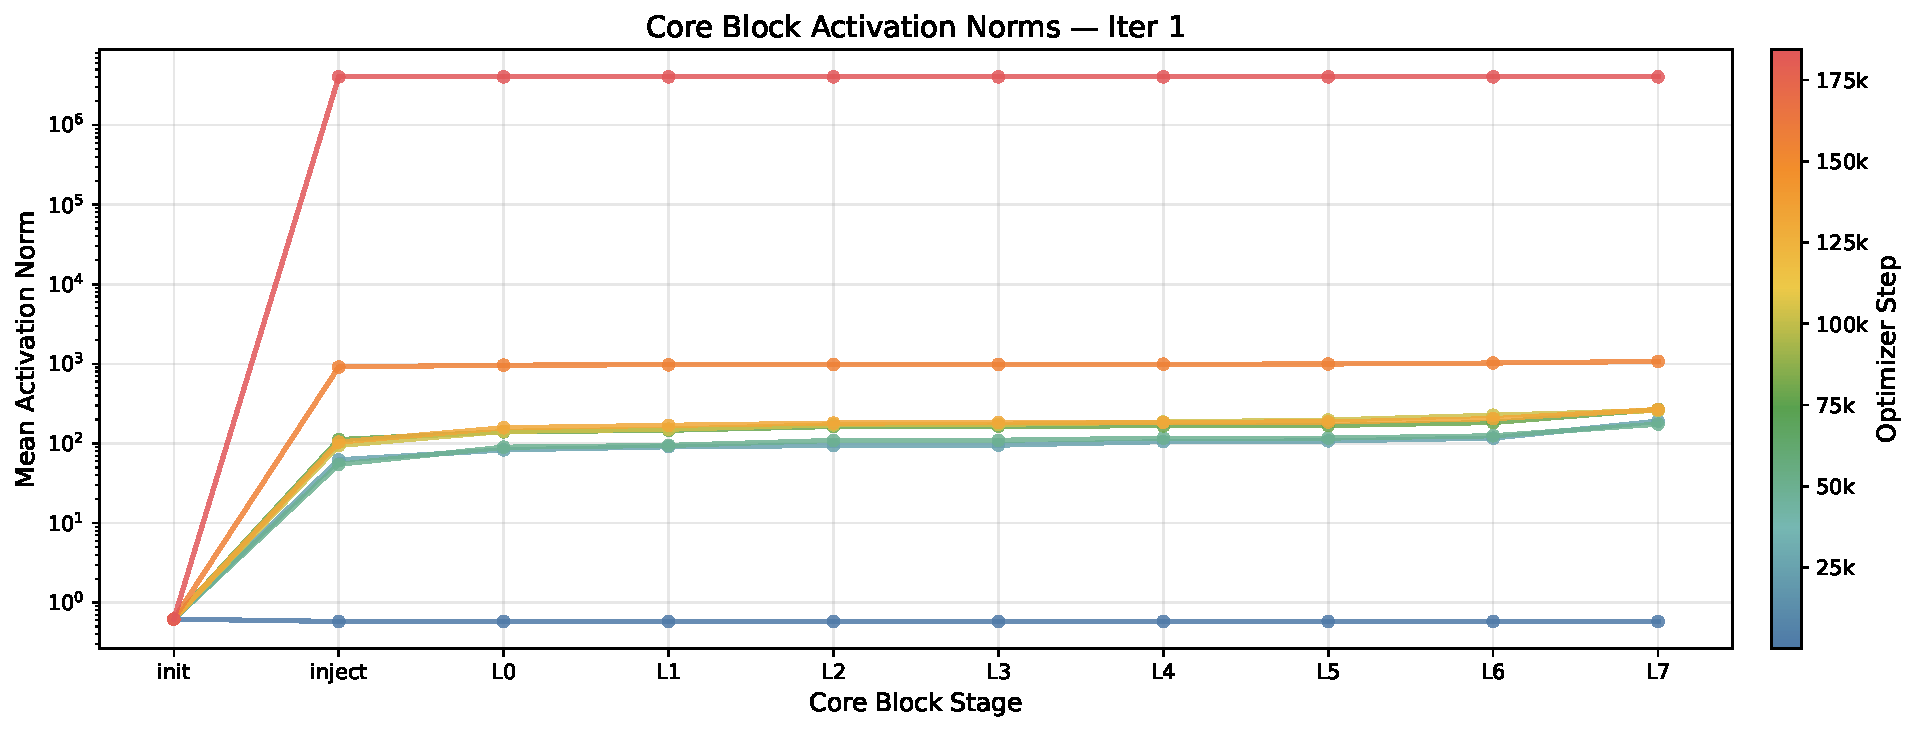
\includegraphics[width=\linewidth]{figures/appendix/core_block_norms.pdf}
    \caption{\textbf{Recurrent State Norm Progression After Each Transformer Block for $T=1$.} For each checkpoint we have for our failed 1.3B Parcae model run, we evaluate the recurrent norm after injection and each non-linear transformer block for only $T=1$. We find that the non-linear parts of Parcae have little effect on explosion, which instead mainly stems from the initial injection of prelude output $e$.}
    \label{fig:injection-explosion}
\end{figure}

\begin{figure}[!t]
    \centering
    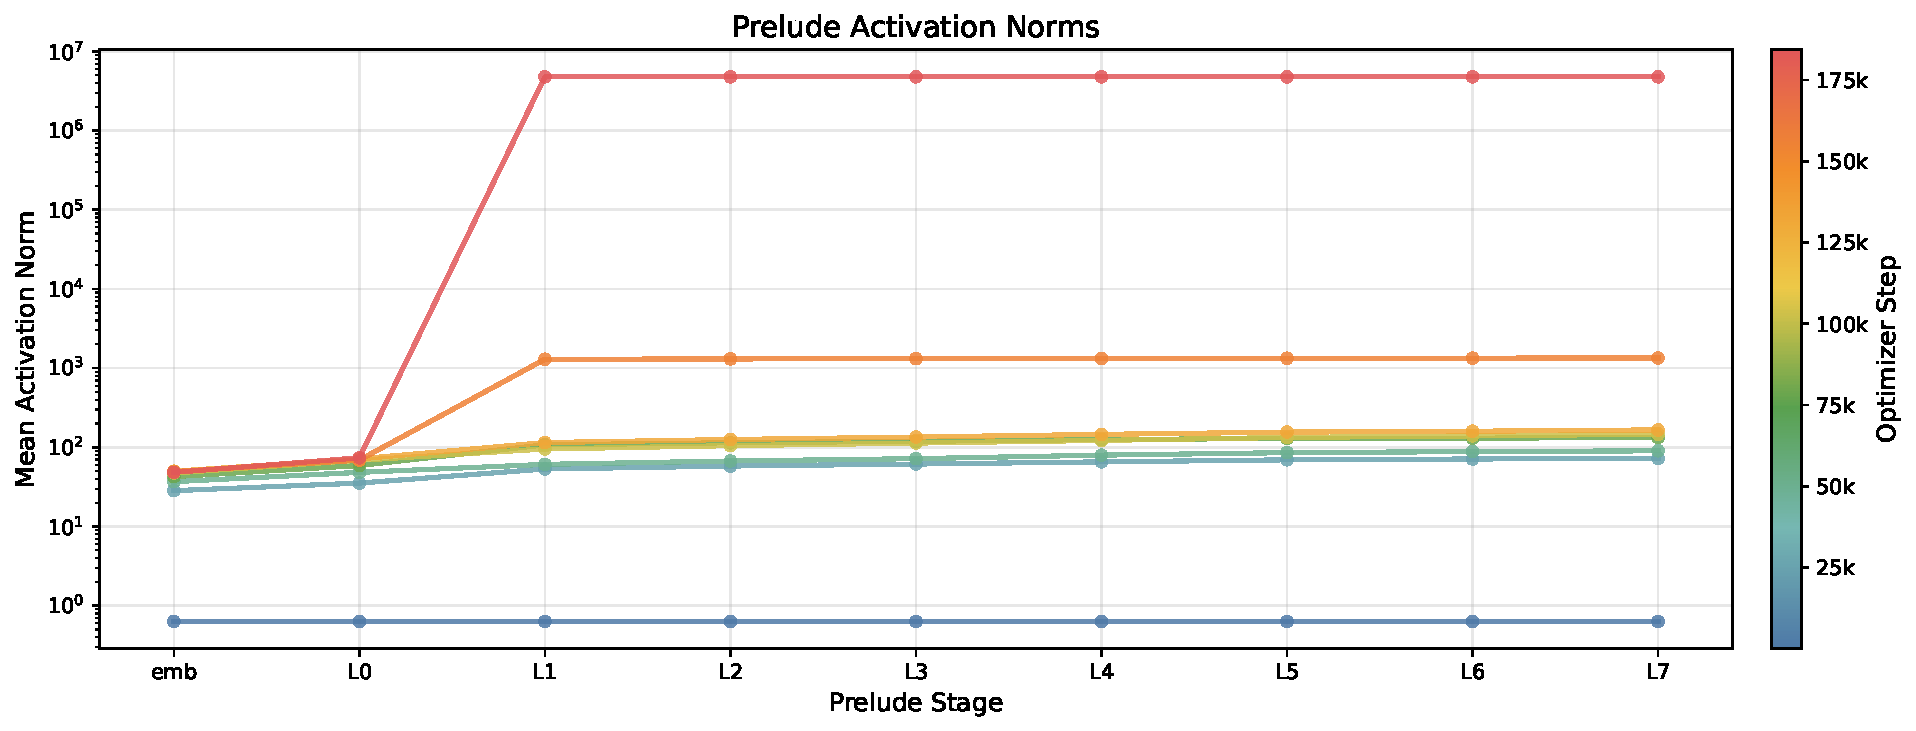
\includegraphics[width=\linewidth]{figures/appendix/prelude_norms.pdf}
    \caption{\textbf{State Norm Progression Throughout each Transformer Layer in the Prelude Block.} For each checkpoint we have for our failed 1.3B Parcae model run, we evaluate residual norm after each transformer block in the prelude \prelude. We find that a single layer creates an explosion of the residual norm and leads to divergence.}
    \label{fig:prelude-explosion}
\end{figure}

Given this, we propose a simple fix of adding a normalization layer on the output of the prelude block \prelude (i.e., for an input $x$ then $e \gets \text{LN}(\mathcal{P}(x))$, where $\text{LN}(\cdot)$ is some form of normalization). We note that this does two things: (1) normalizes the input to the recurrent unit, which we observe to further stabilize the recurrent dynamics of looping, and (2) stabilizes the gradient flow to the \prelude.\footnote{We do not directly prove or show this; however, it can be inferred by prior work on how normalization stabilizes forward and backward passes of transformers \cite{xu2019understandingimprovinglayernormalization, xiongLayerNormalizationTransformer2020}.} This simple fix enables our stable training run for the 1.3B Parcae reported in \cref{sec:results}.


Empirically, we find that using a prelude norm directly stabilizes the recurrent norm further, preventing the recurrent norm from growing too large (see \cref{fig:prelude-norm-better}). Additionally, we find that using a prelude norm leads to better convergence in both our 140M and 370M Parcae models (see \cref{fig:prelude-quality}), with only a negligible improvement for our 770M and 1.3B Parcae models.

\begin{figure}[!h]
    \centering
    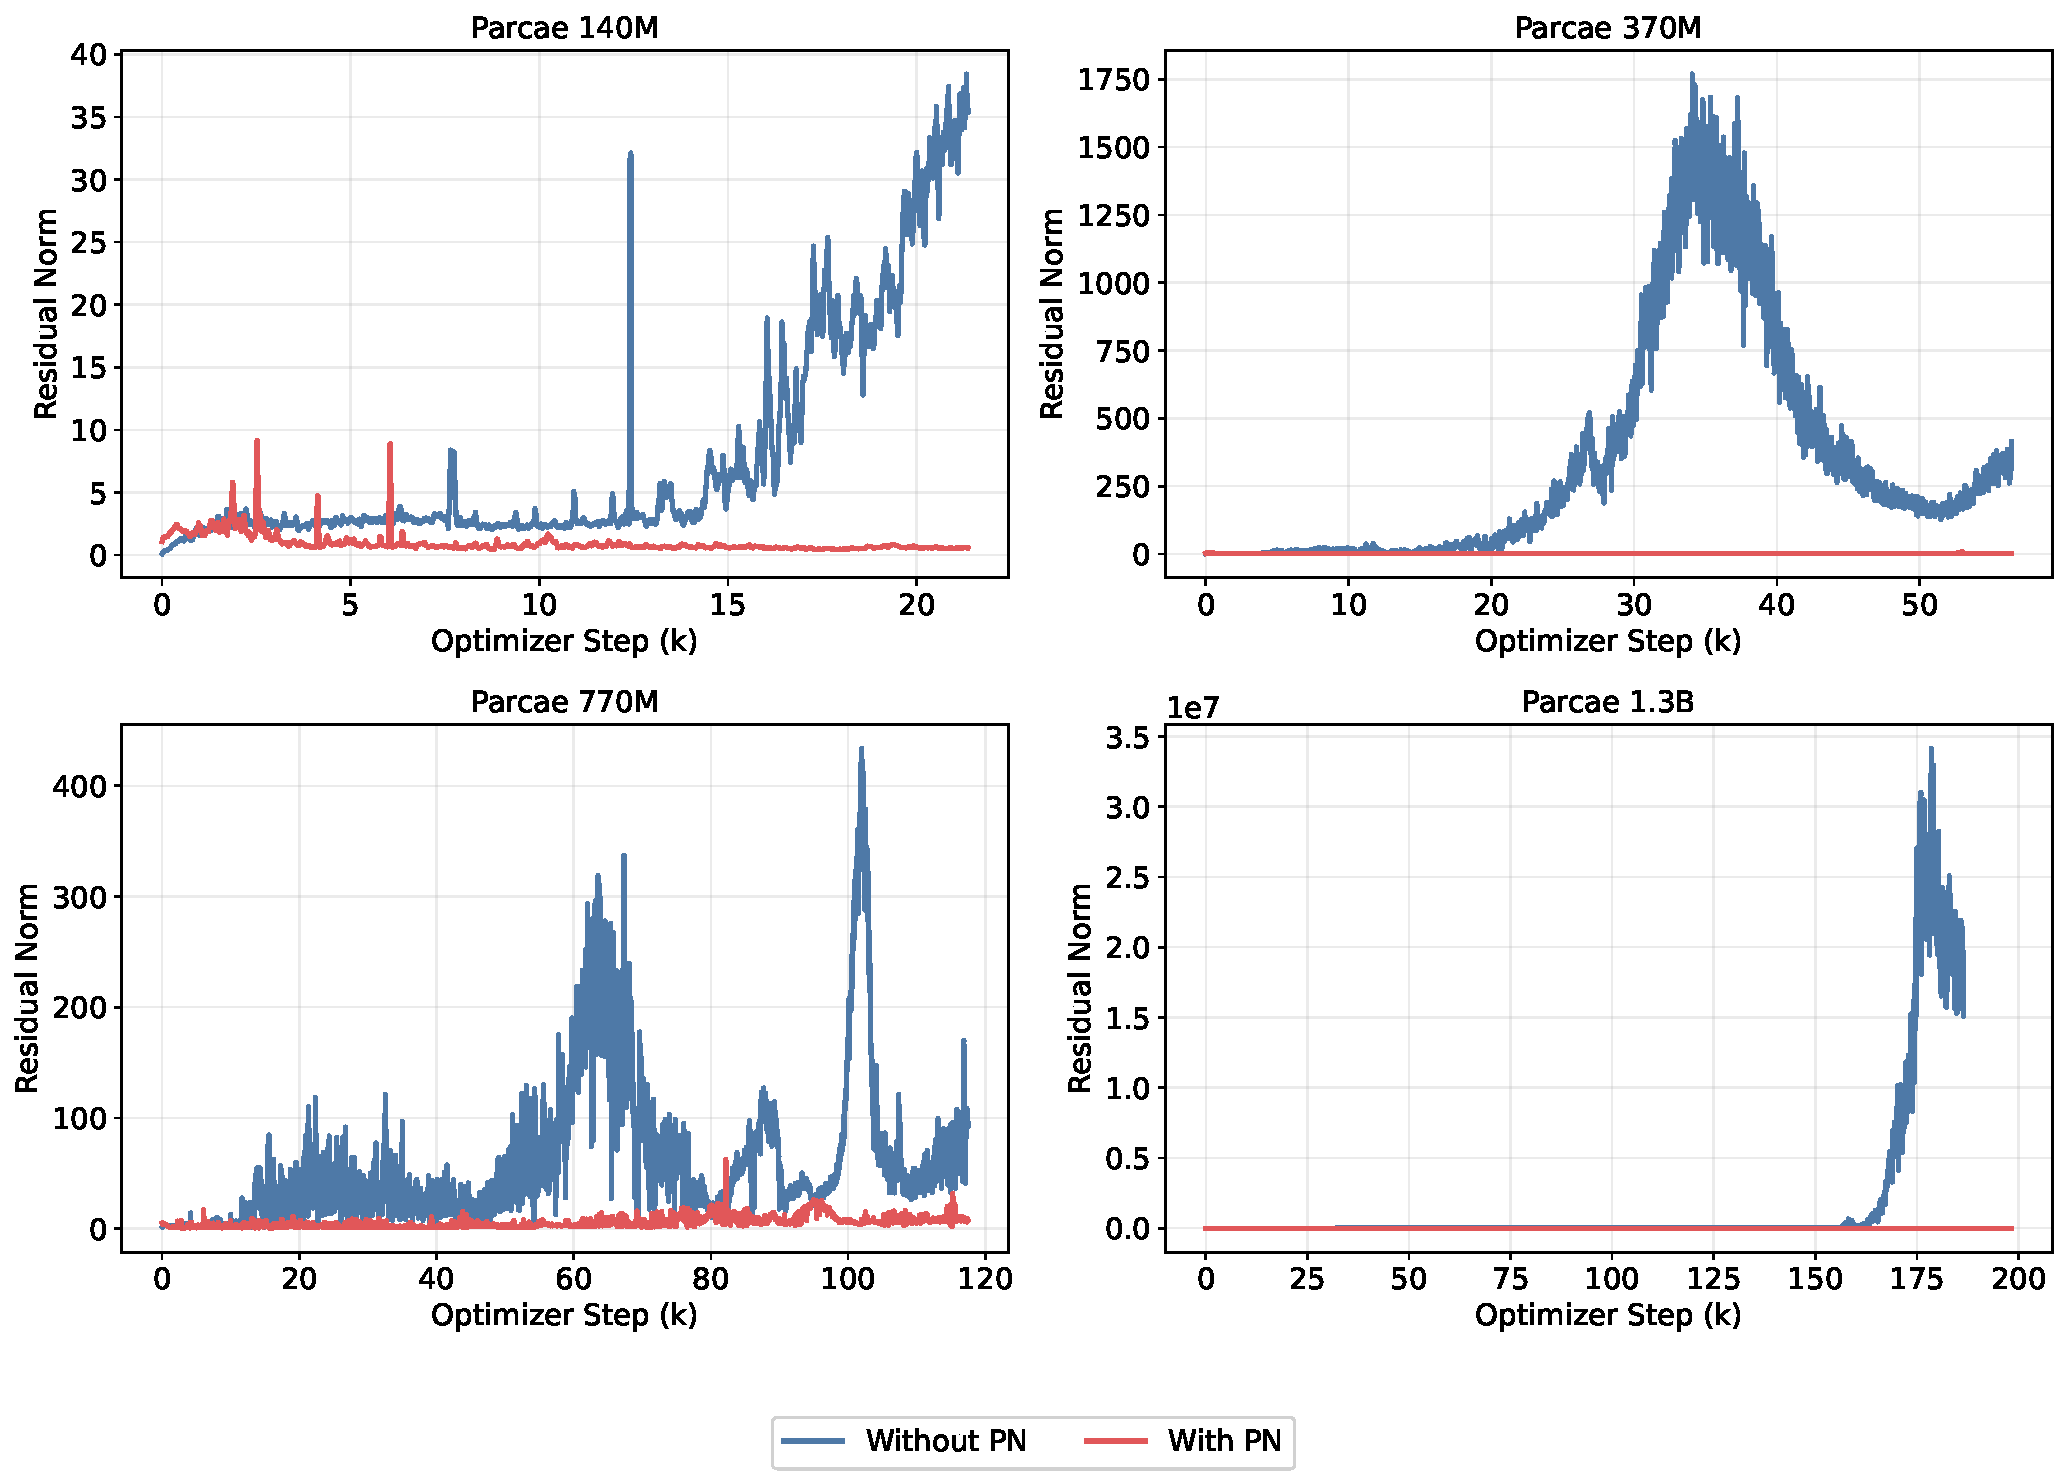
\includegraphics[width=\linewidth]{figures/appendix/prelude_norm_ablation.pdf}
    \vspace{-1em}
    \caption{\textbf{Prelude Norm Stabilizes Recurrent Norm.} We find that prelude norm helps stabilize recurrent state norm in Parcae models following the setup in \cref{sec:e2e} for Transformers.}
    \label{fig:prelude-norm-better}
\end{figure}


\begin{figure}[!h]
    \centering
    \vspace{-1em}
    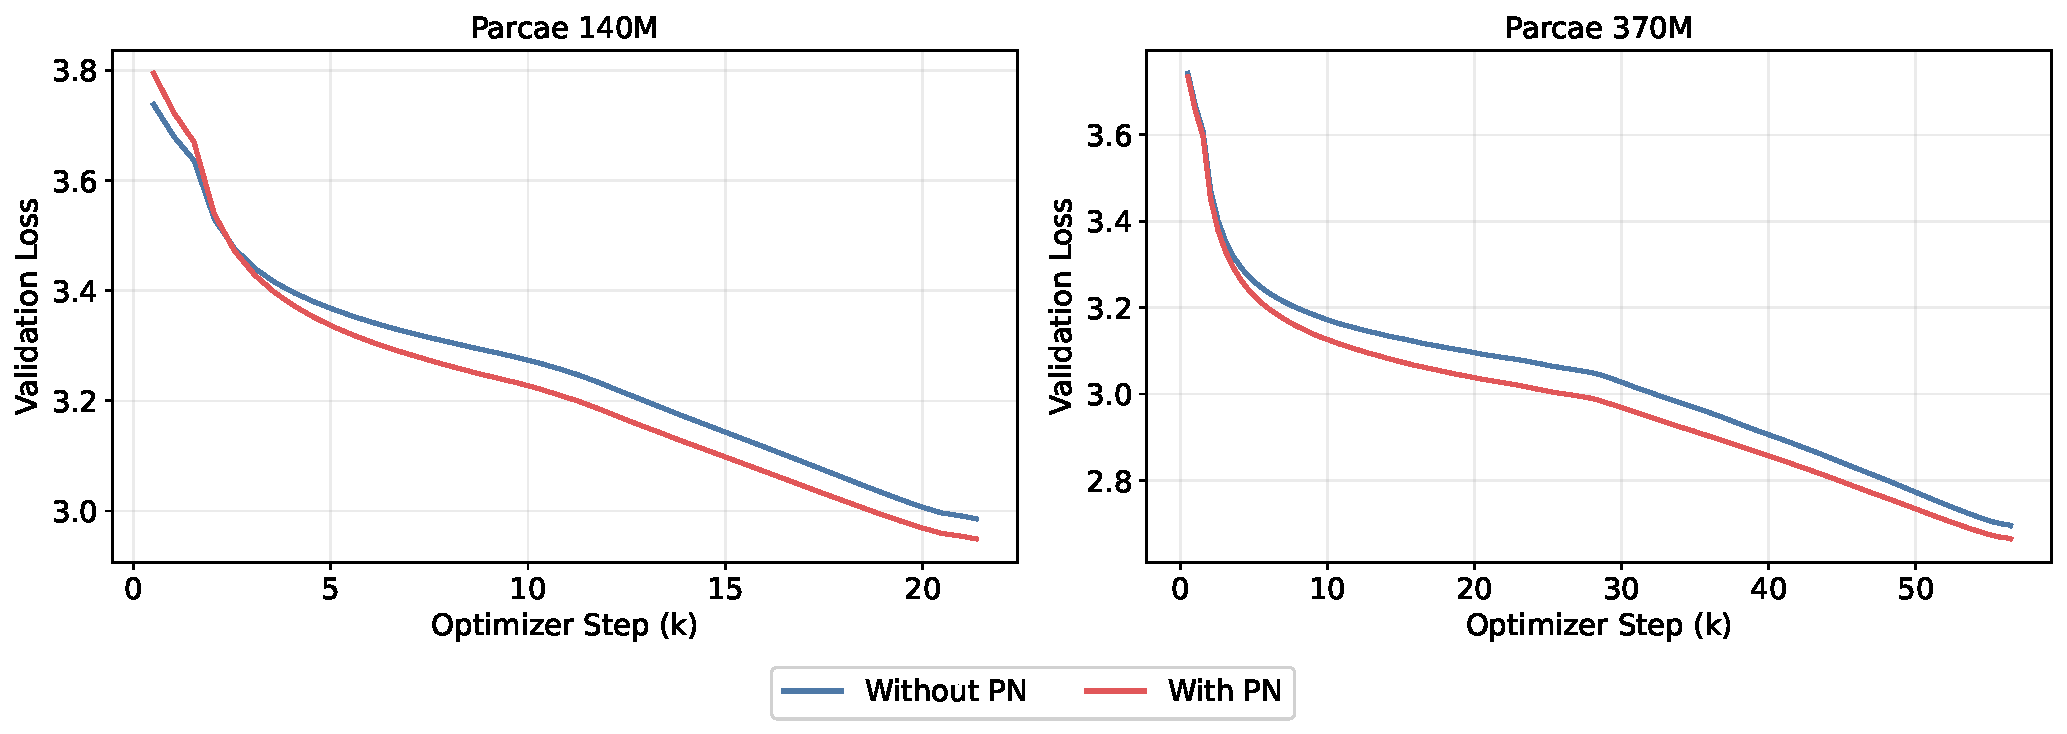
\includegraphics[width=\linewidth]{figures/appendix/prelude_norm_val_loss.pdf}
    \vspace{-1em}
    \caption{\textbf{Prelude Norm Improves Quality.} We find that in our 140M and 370M Parcae models trained in the same setup as \cref{sec:e2e} for Transformers, normalizing the prelude output leads to better convergence.}
    \label{fig:prelude-quality}
\end{figure}
